\documentclass[tikz,border=8pt]{standalone}
\usepackage[T1]{fontenc}
\usepackage[utf8]{inputenc}
\usepackage[sc]{mathpazo}
\usepackage{amsmath,amssymb}
\usepackage{xcolor}
\usepackage{tikz}
\usetikzlibrary{arrows.meta,calc,positioning,fit,backgrounds,decorations.pathmorphing}

\definecolor{cmjcrimson}{RGB}{155,20,30}
\definecolor{cmjgold}{RGB}{186,145,40}
\definecolor{cmjdark}{RGB}{35,35,35}
\definecolor{cmjgray}{RGB}{128,128,128}

\begin{document}
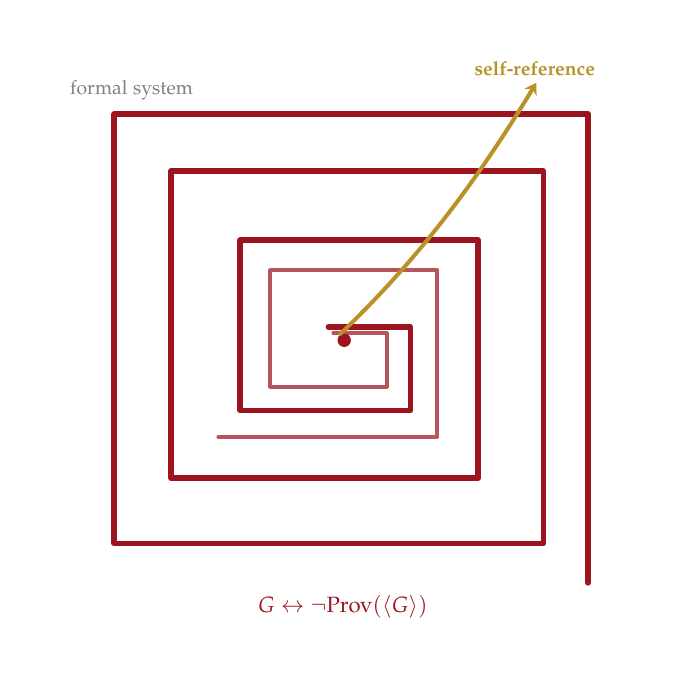
\begin{tikzpicture}[>=Stealth, line cap=round, line join=round, font=\small]
   \path[use as bounding box] (-4,-4) rectangle (4,4); % square canvas only
   % Title: Self-Reference and Incompleteness
   % Figure illustrates a formal proof system whose internal encoding creates a statement escaping total completeness.
   % no rendered title at the top
   % no visible frame box, no dashed guide frame, no center crosshair

   \draw[cmjcrimson, line width=2.05pt]
      (-0.18,0.20) -- (0.86,0.20) -- (0.86,-0.86) -- (-1.30,-0.86)
      -- (-1.30,1.30) -- (1.72,1.30) -- (1.72,-1.72) -- (-2.18,-1.72)
      -- (-2.18,2.18) -- (2.55,2.18) -- (2.55,-2.55) -- (-2.90,-2.55)
      -- (-2.90,2.90) -- (3.12,2.90) -- (3.12,-3.05);

   \draw[cmjcrimson, line width=1.30pt, opacity=0.72]
      (-0.12,0.12) -- (0.56,0.12) -- (0.56,-0.56) -- (-0.92,-0.56)
      -- (-0.92,0.92) -- (1.20,0.92) -- (1.20,-1.20) -- (-1.58,-1.20);

   \fill[cmjcrimson] (0.02,0.03) circle (0.085);

   \draw[cmjgold, line width=1.45pt, -{Stealth[length=4pt,width=5pt]}]
      (-0.03,0.11) .. controls (0.92,1.02) and (1.66,1.98) .. (2.46,3.3);

   \node[cmjgray, font=\scriptsize] at (-2.68,3.2) {formal system};
   \node[cmjgold, font=\scriptsize\bfseries] at (2.44,3.48) {self-reference};
   \node[cmjcrimson, font=\footnotesize] at (0,-3.35) {$G \leftrightarrow \neg\mathrm{Prov}(\langle G\rangle)$};

\end{tikzpicture}
\end{document}
